\clearpage

\chapter{Use Case Diagramme}
Folgend wird die Software als Use Case Diagramme dargestellt. Use Case Diagramme stellen das System von außen dar. ............................................

\section{Spieler verwalten - $\backslash$LF10$\backslash$,$\backslash$LF11$\backslash$,$\backslash$LF12$\backslash$}
\begin{figure}[!h]
	\centering
    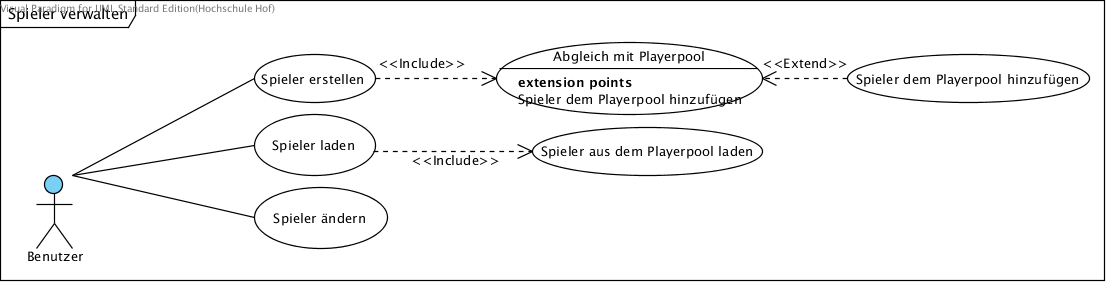
\includegraphics[width=\textwidth]{./SpielerVerwalten.png}
	\label{layout_gesamt}
\end{figure}

\clearpage
\section{Anzahl der Spieler wählen - $\backslash$LF20$\backslash$}
\begin{figure}[!h]
	\centering
    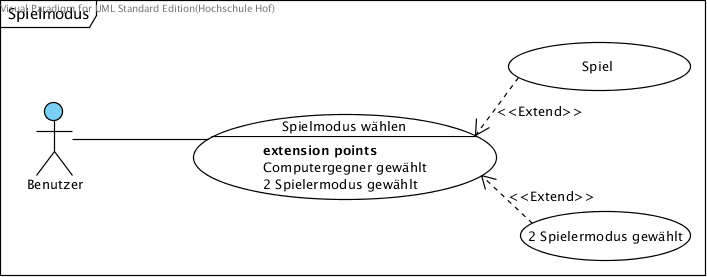
\includegraphics[width=\textwidth]{./AnzahlSpieler.png}
	\label{layout_gesamt}
\end{figure}

\clearpage
\section{Thema wählen - $\backslash$LF30$\backslash$}
\begin{figure}[!h]
	\centering
    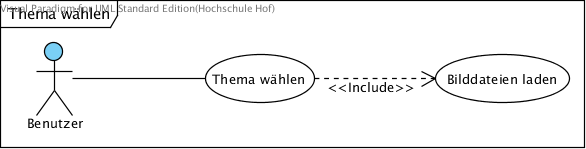
\includegraphics[width=\textwidth]{./Thema.png}
    
	\label{layout_gesamt}
\end{figure}

\clearpage
\section{Spielfeldgröße wählen - $\backslash$LF40$\backslash$}
\begin{figure}[!h]
	\centering
    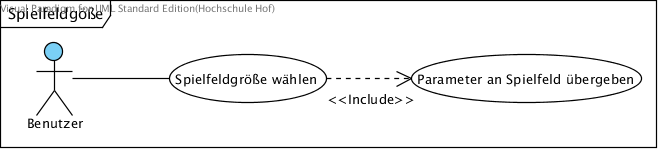
\includegraphics[width=\textwidth]{./Spielfeldgroesse.png}
	\label{layout_gesamt}
\end{figure}

\clearpage
\section{Spiel starten - $\backslash$LF50$\backslash$}
\begin{figure}[!h]
	\centering
    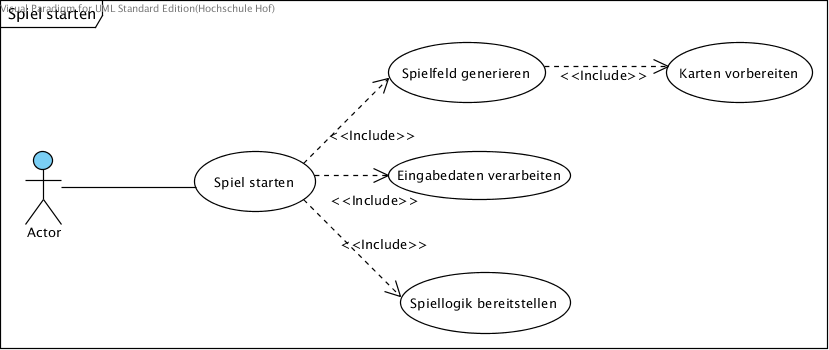
\includegraphics[width=\textwidth]{./SpielStarten.png}
	\label{layout_gesamt}
\end{figure}

\clearpage
\section{Highscore - $\backslash$LF60$\backslash$,$\backslash$LF61$\backslash$}
\begin{figure}[!h]
	\centering
    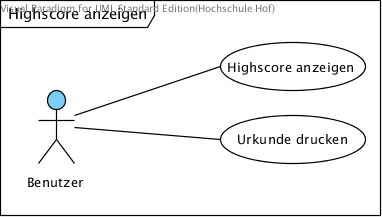
\includegraphics[width=\textwidth]{./Highscore.png}
	\label{layout_gesamt}
\end{figure}

\clearpage
\section{Vokabeltraining - $\backslash$LF70$\backslash$}
\begin{figure}[!h]
	\centering
    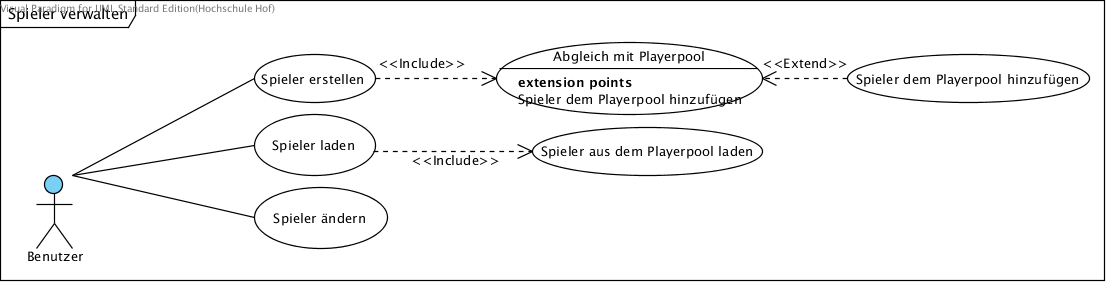
\includegraphics[width=\textwidth]{./SpielerVerwalten.png}
	\label{layout_gesamt}
\end{figure}

\clearpage
\section{Audiodaten abspielen - $\backslash$LF80$\backslash$}
\begin{figure}[!h]
	\centering
    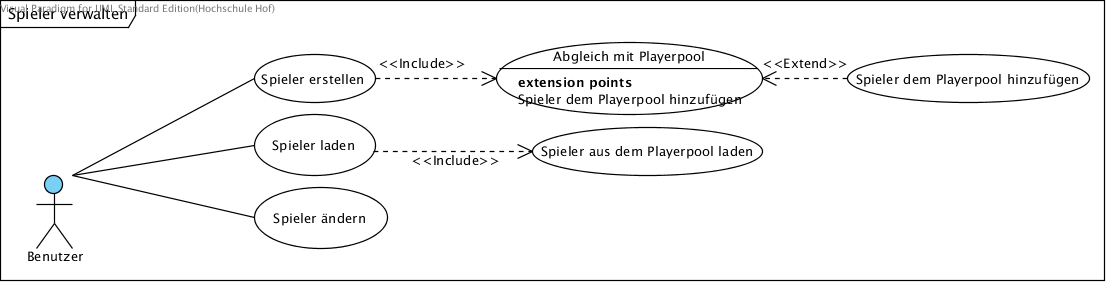
\includegraphics[width=\textwidth]{./SpielerVerwalten.png}
	\label{layout_gesamt}
\end{figure}

